\documentclass[10pt]{beamer}

\usepackage[style=british]{csquotes}
\usepackage{graphicx}

\usepackage{caption}
\usepackage{subcaption}
\usepackage{xcolor}
\usepackage[lined,boxed]{algorithm2e}



\usetheme[progressbar=frametitle]{metropolis}
\usepackage{appendixnumberbeamer}

\usepackage{booktabs}
\usepackage[scale=2]{ccicons}

\usepackage{pgfplots}
\usepgfplotslibrary{dateplot}

\usepackage{xspace}
\newcommand{\themename}{\textbf{\textsc{metropolis}}\xspace}

\title{Hider/Finder/Combiner}
\subtitle{A new approach to machine learning-based speech control}
% \date{\today}
\date{}
\author{Jacob Josiah Webber}
\institute{Centre for Speech Technology Research}
\titlegraphic{\hfill
\includegraphics[height=1.5cm]{logo.pdf}}

\begin{document}

\maketitle

\begin{frame}{Table of contents}
  \setbeamertemplate{section in toc}[sections numbered]
  \tableofcontents[hideallsubsections]
\end{frame}

\section{Introduction}

\begin{frame}[fragile]{Why are we here?}
%We present a new way of using neural networks to control speech.

In this talk I will
\begin{itemize}
    \item describe an ideal controllability,
    \item demonstrate how machine learning can be not well suited to creating controllable systems,
    \item show a novel neural architecture for overcoming this, and
    \item show the results of my implementation and experiments.
\end{itemize}
\end{frame}

\section{Describing Controllability}

\begin{frame}{Controlling A Speech Signal}
What does it \emph{REALLY} mean to control one (or many) aspect/s of a speech signal...
\end{frame}

\begin{frame}{Parameter Decomposition}
There are lots of ways to represent a speech signal...
\begin{itemize}
    \item We can measure parameters from a speech signal
    \item For example, F0, Question?, spectral tilt...
    \item We want to be able to modify these parameters
    \item We want to change as few parameters as possible in the original signal, only changing a control parameter.
\end{itemize}{}
Many of the parameters we wish to modify are deeply intertwined/interdependent with others.
\end{frame}{}


\begin{frame}{De-interdependence}

We want to keep all the parameters the same that are not dependent on the control parameter
\begin{itemize}
    \item E.g., how do we keep spectral tilt the same when modifying F0?
    \item Is this desirable? Probably not
    \item Spectral tilt is part speaker characteristics, part F0.
    \item Need to separate parts of non-control variables that are not dependent on control parameter
\end{itemize}{}
Sometimes it is possible to do this analytically, using signal processing methods.
\end{frame}{}

\section{Controllability and Machine Learning}
\begin{frame}[fragile]{The Problem}
We want to be able to modify a speech signal by an arbitrary \emph{control parameter}.

This is \emph{hard} using existing machine learning techniques.

%\begin{itemize}
%    \item Machine learning to control a parameter requires a set of datapoints with same content but different values of control parameter
%    \item Similar to parallel texts for NMT
%    \item 
%\end{itemize}


\end{frame}

\begin{frame}{Machine Learning -- Overview}
    Neural networks are \emph{universal function approximators}
    \begin{equation}
        z = f(x)
    \end{equation}
    Say, $x$ is magnitude spectrum and $z$ is waveform.
    Can map between two with network $F$
    \begin{equation}
        z \approx F(x)
    \end{equation}
    Learn to do this -- backprop through error $\epsilon$
    \begin{equation}
        \epsilon = f(x) - F(x)
    \end{equation}
    for all $(x,z)$ in some training set.
\end{frame}

\begin{frame}{Adaptable by Parameter? No}
We want to modify some parameter $y$ in the speech signal. We choose F0.

Add it as input param?
\begin{equation}
    z \approx F(x,y)
\end{equation}
	\begin{alertblock}{Network ignores $y$!}
	$x$ contains all the necessary information about $y$ to derive $z$.
	
	If we change $y$, this information will contradict $x$
	\end{alertblock}
\end{frame}

\begin{frame}{Adaptable? Yes}
Instead derive a hidden representation which contains as little information as possible about $y$, but all other information necessary to combine with $y$ to form $z$.

We use a \emph{hider} ($H$) 
\begin{equation}
    h = H(x)
\end{equation}
and \emph{combiner} ($C$) network for this
\begin{equation}
    z \approx C(h,y)
\end{equation}
with a \emph{finder} ($D$) adversary
\begin{equation}
    y \approx D(h)
\end{equation}
\end{frame}

\begin{frame}[fragile]{Training Adversarially}
    \begin{figure}[h]
    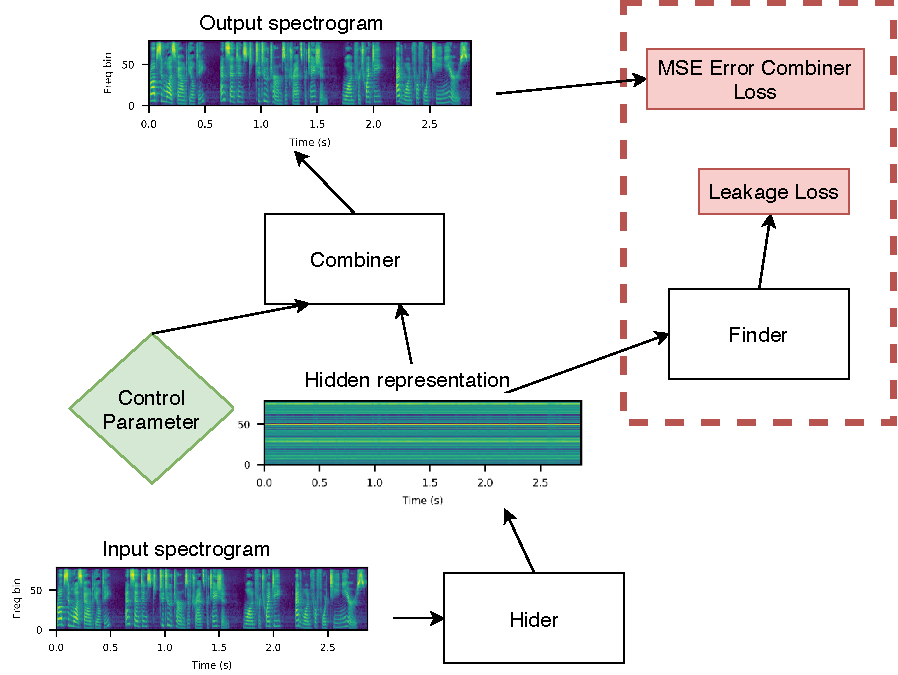
\includegraphics[width=0.72\textwidth]{figures/adversarial-training.pdf}
  \caption{The complete architecture. Components in the dashed box are used only during training.}
  \label{fig:adverse-over}
\end{figure}
\end{frame}

\begin{frame}[plain]
 \begin{figure}[h]
    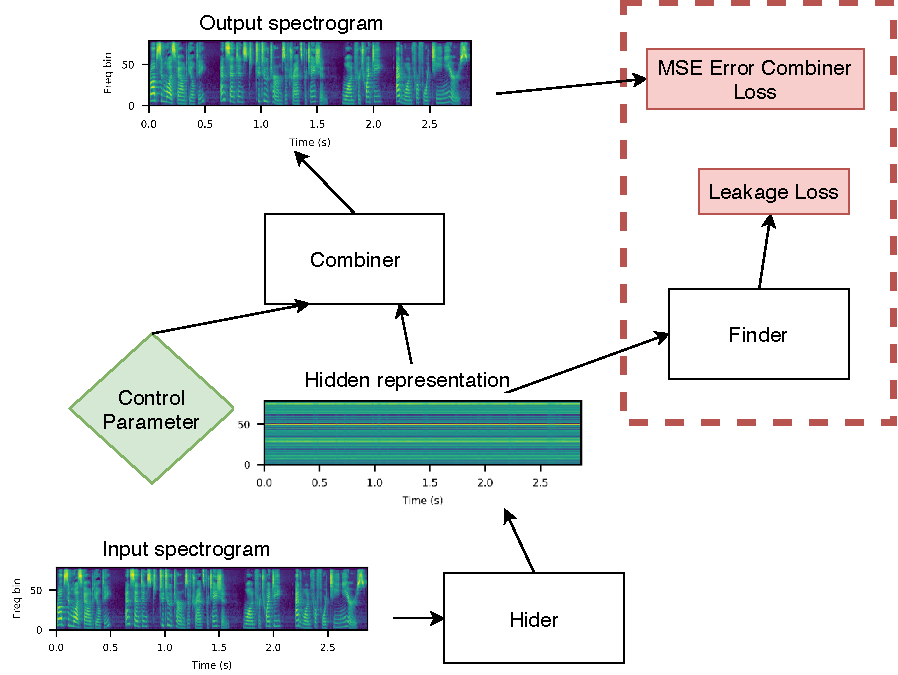
\includegraphics[width=1\textwidth]{figures/adversarial-training.pdf}
  \end{figure}
\end{frame}

\begin{frame}[fragile]{Algorithm: Two-step update process}
Experiments were done modifying F0

We train the system over two steps -- first generate a hidden representation and use this to train Finder

Then train rest of system with composite loss function for leakage loss and combiner loss

\end{frame}

\begin{frame}[fragile]{Algorithm: Two-step update process}
\IncMargin{1em}
\begin{algorithm}[H]
\small
  \KwData{For each speech sample in the dataset: mel-spectrogram and F0 values}
  \KwResult{Trained network parameters}
  \ForEach{speech sample}{
     \tcc{First train finder network}
  	Generate hidden state by passing mel-spect into hider network\;
  	Use finder network on hidden state to get estimated F0\;
  	Calculate cross-entropy loss between estimated F0 and F0\;
  	Backprop through finder parameters and update\;
  	\tcc{Train hider and combiner}
  	Pass F0 and hidden state into combiner\;
  	Calculate MSE combiner loss and leakage loss, sum\;
  	Backprop loss through \emph{both} hider \emph{and} combiner parameters\;
  	Update combiner and hider parameters using Adam optimiser\;
  }
 \caption{Training algorithm for adversarial training}
  \label{alg:adv}
\end{algorithm}
\end{frame}

\begin{frame}[fragile]{Component architecture}
\begin{figure}[h]
  \centering
	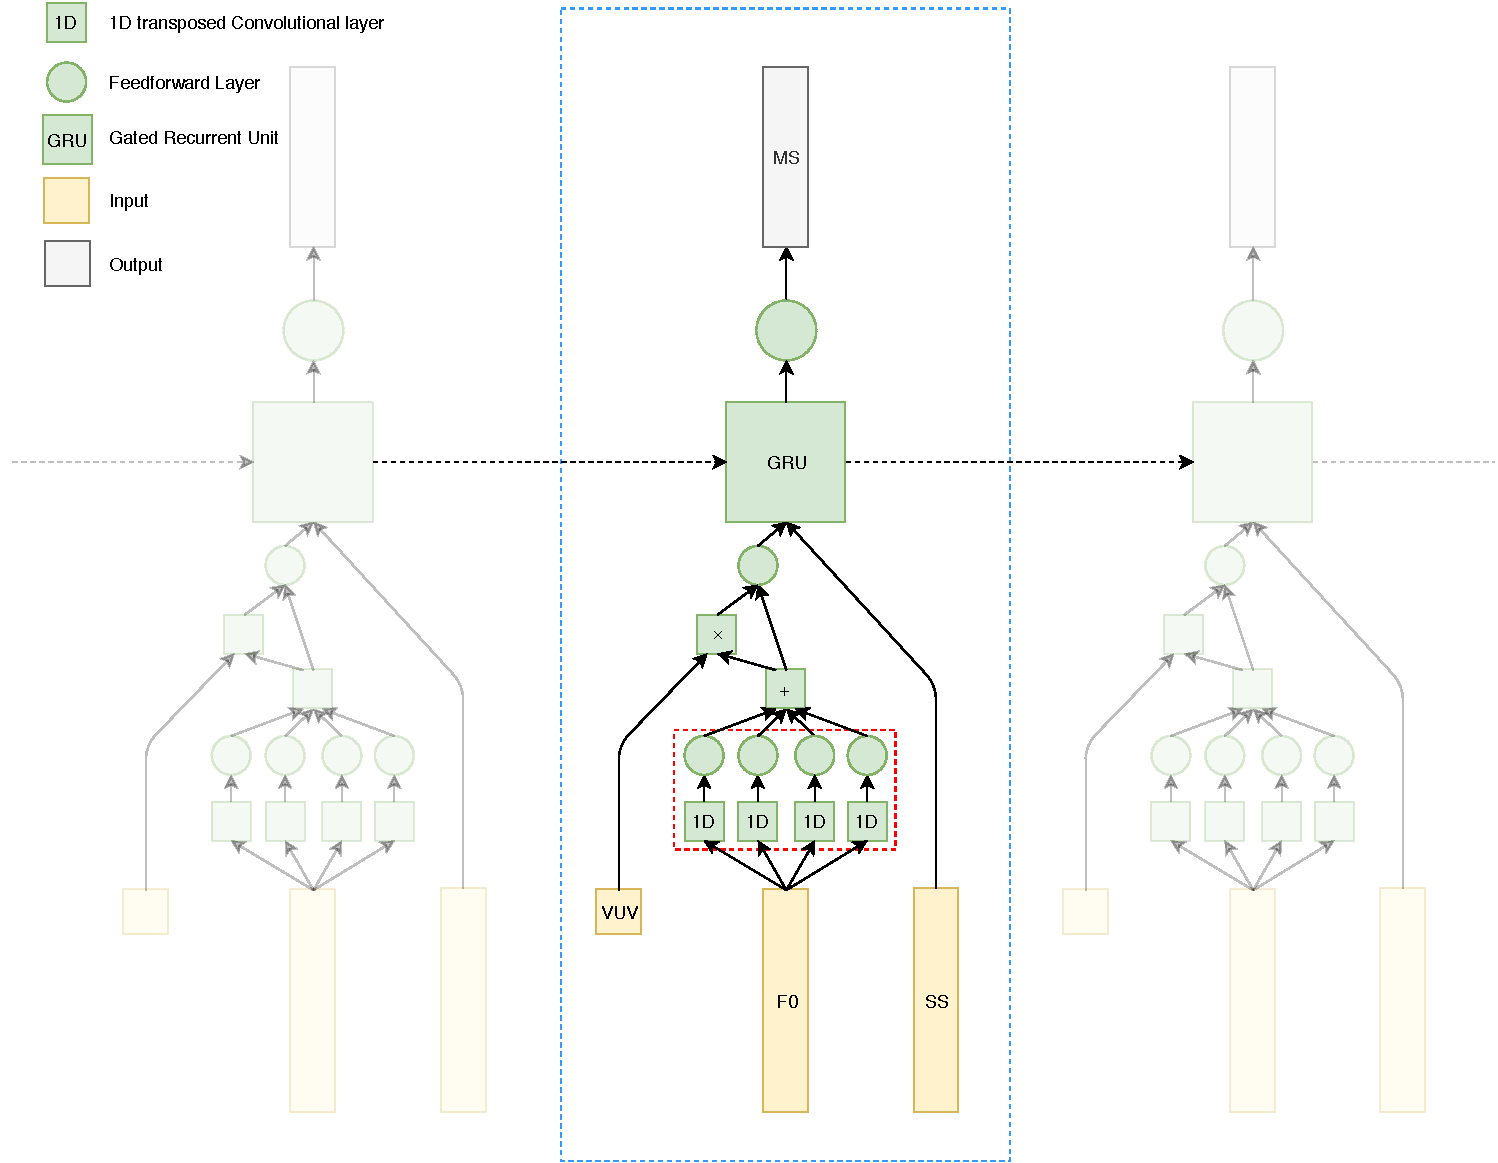
\includegraphics[width=0.68\textwidth]{figures/combining-network-crop} 
  \caption{Combiner Network. A lot of detail is omitted -- all networks are recurrent and fairly sophisticated}
\label{comb-diag}
\end{figure}
\end{frame}

\begin{frame}[plain]
\begin{figure}[h]
  \centering
	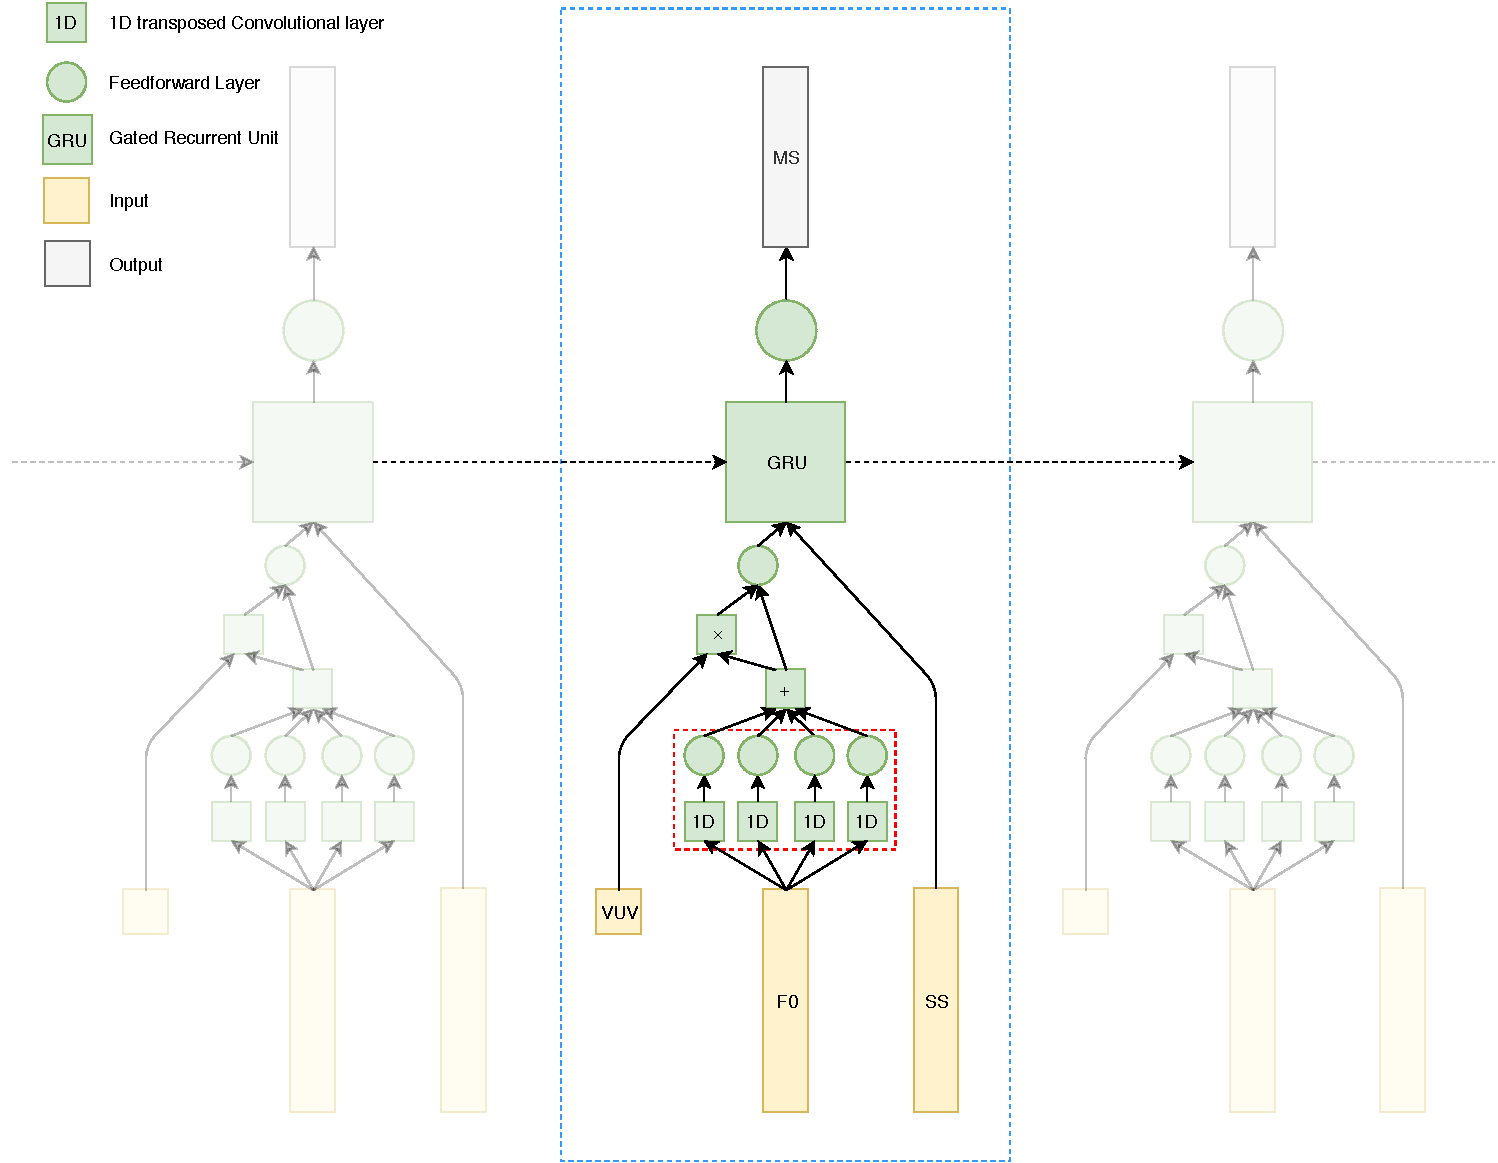
\includegraphics[width=1\textwidth]{figures/combining-network-crop}
\label{comb-diagbig}
\end{figure}
\end{frame}

\section{Results}

\begin{frame}{Details}
For experiments...
\begin{itemize}
    \item System took magnitude spectrum as input. Gives magnitude spectrum as output
    
    \item Use Amazon Universal Vocoder to generate audio.
    
    \item Use F0 (pitch) as control variable.
    
    \item Use \emph{World} as baseline. Ran listening test
    
    \item World is preferred 92\% of the time. \textcolor{red}{Negative result!}
    
    \item I will play you some audio
\end{itemize}

\begin{alertblock}{Conclusion}
Degrades quality more than World, but is passable and does modify F0 successfully.
\end{alertblock}
\end{frame}

\begin{frame}{Leakage Matters}
    \begin{figure}[h]
  \begin{subfigure}[b]{0.28\textwidth}
    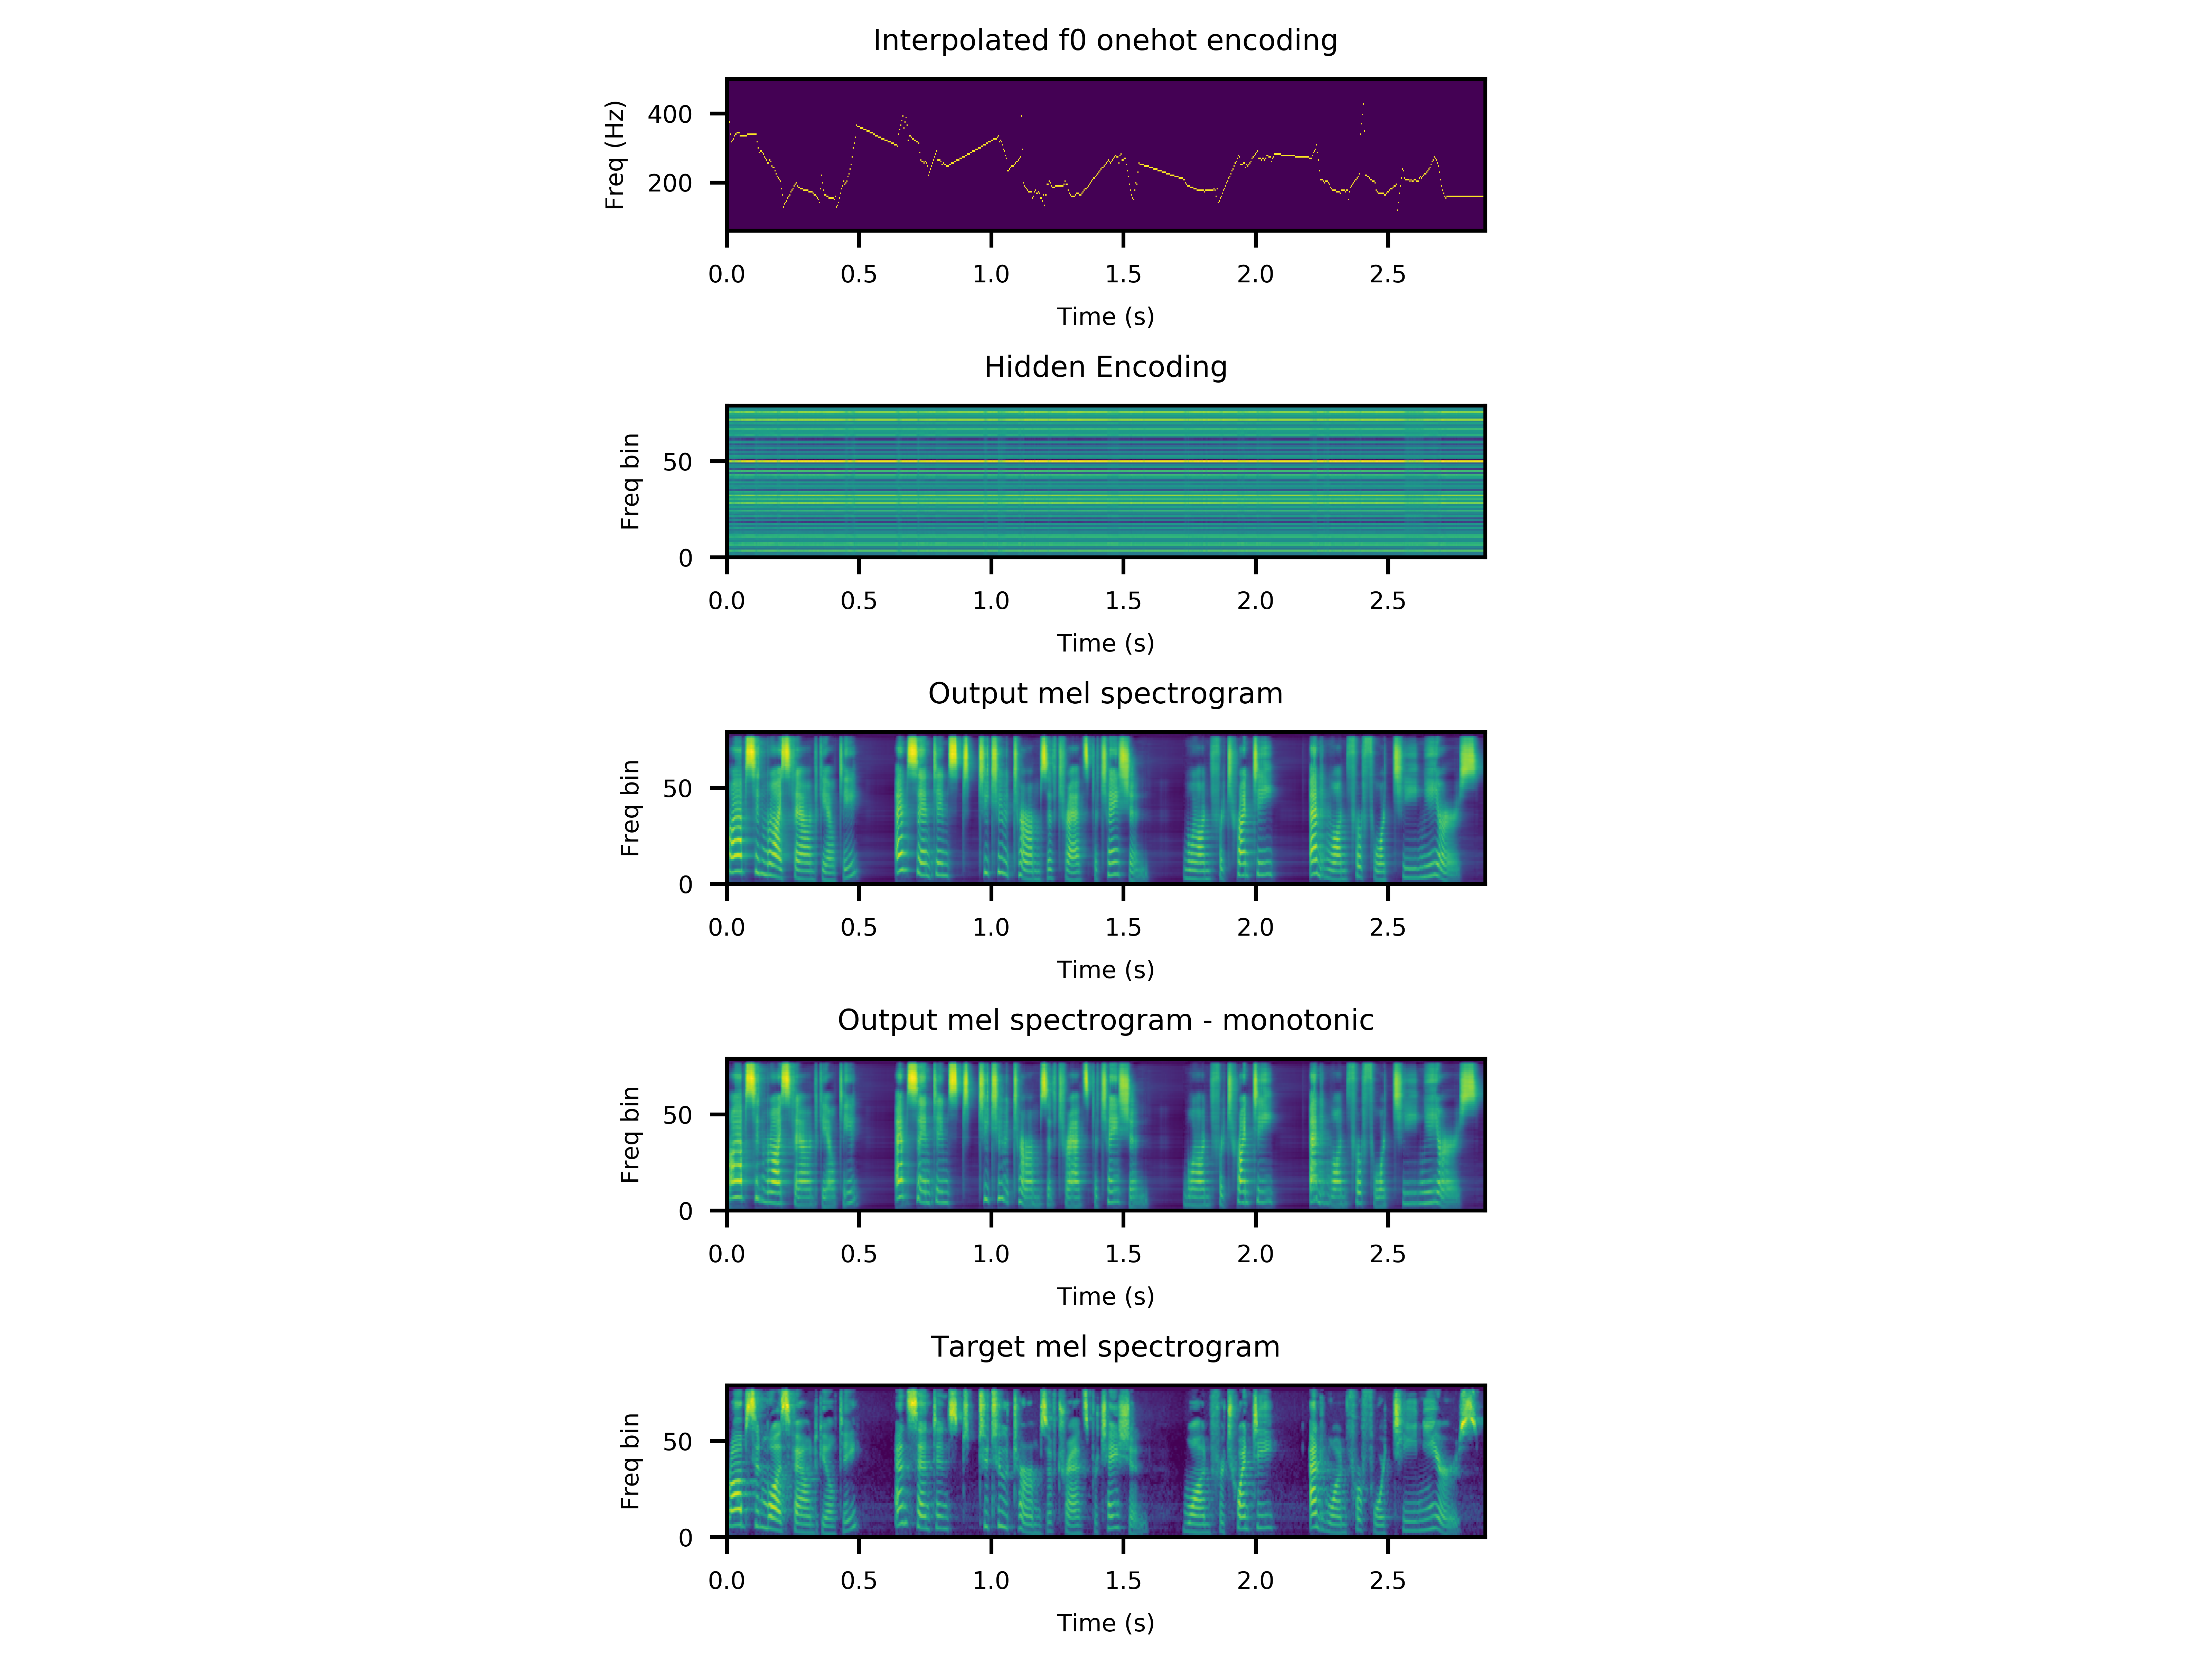
\includegraphics[width=\textwidth,trim={3.8cm 0 4.8cm 0},clip]{figures/beta-100-spects_step-12750-0y0939.png}
    \caption{$\beta$ = 200}
    \label{fig:1beet}
  \end{subfigure}
  %
  \begin{subfigure}[b]{0.28\textwidth}
    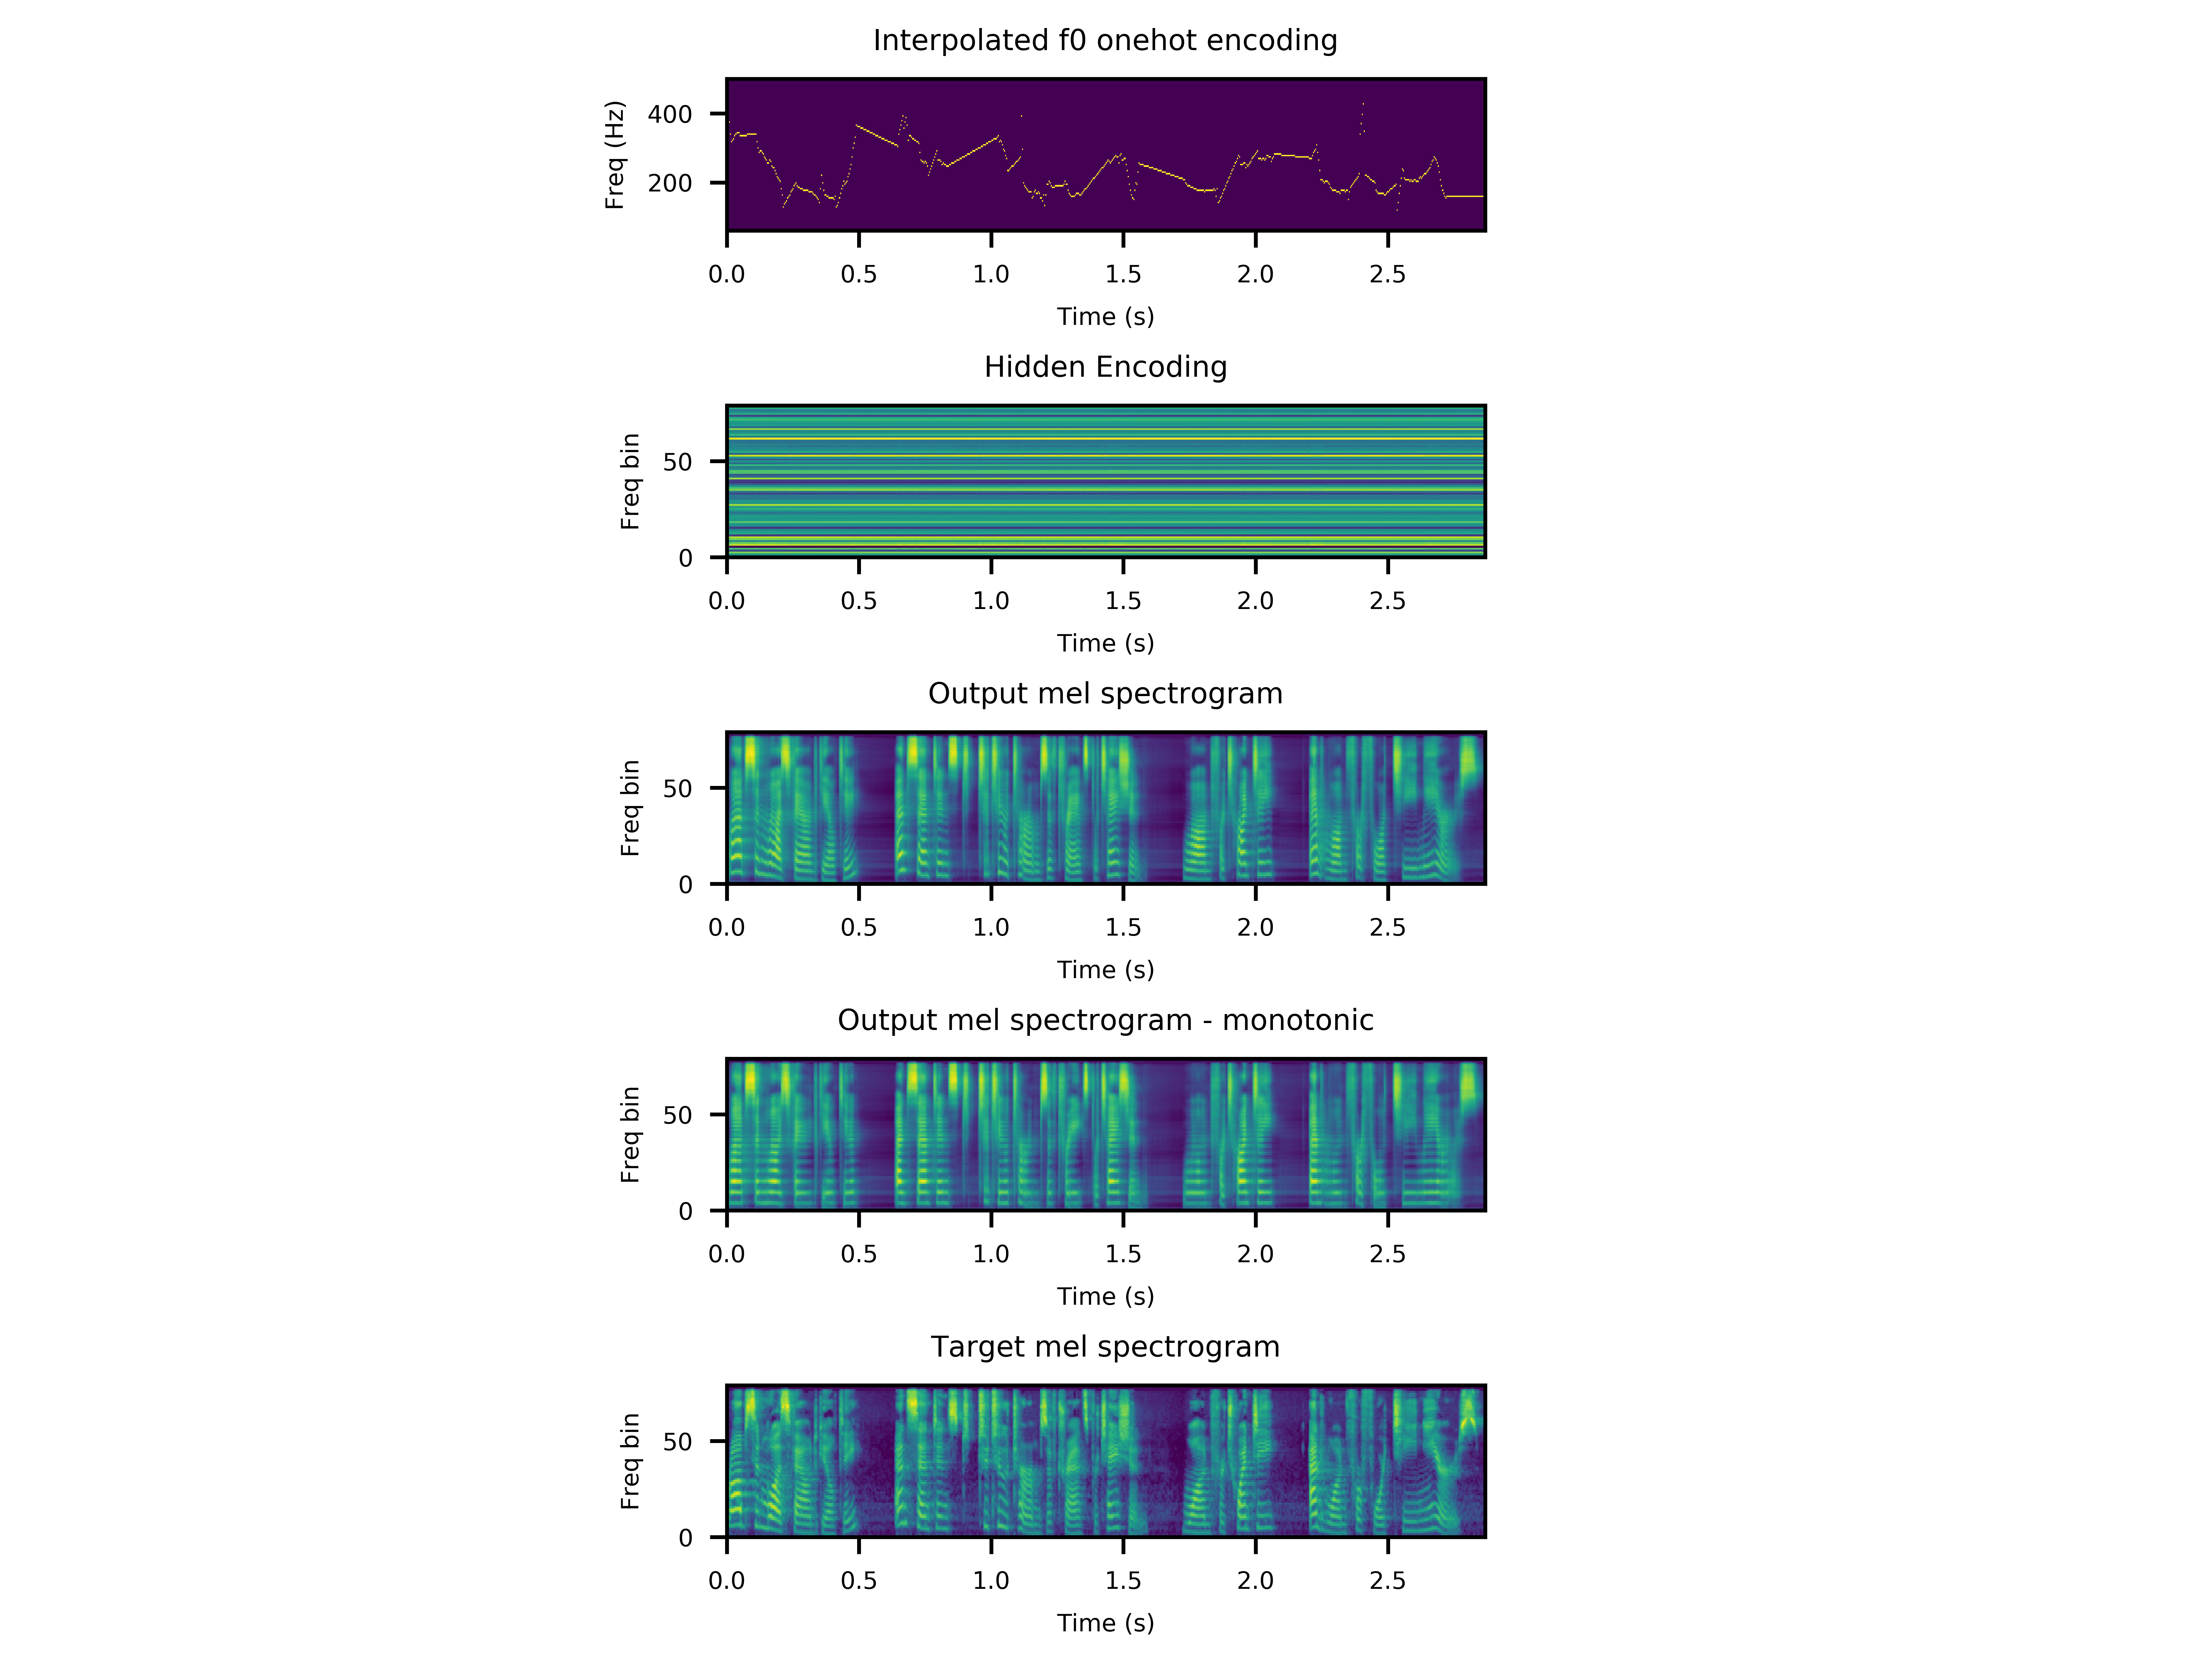
\includegraphics[width=\textwidth,trim={3.8cm 0 4.8cm 0},clip]{figures/beta-800-spects_step-12900-0y1095.png}
    \caption{$\beta$ = 800}
    \label{fig:2}
  \end{subfigure}
  \caption{Figures showing spectrograms for different leakage loss weightings. The monotonic output shown in \ref{fig:1beet} shows clear traces of the original F0.}
  \label{fig:beta-spects}
\end{figure}

\end{frame}



\begin{frame}[plain]
    \begin{figure}[h]
  \begin{subfigure}[b]{0.45\textwidth}
    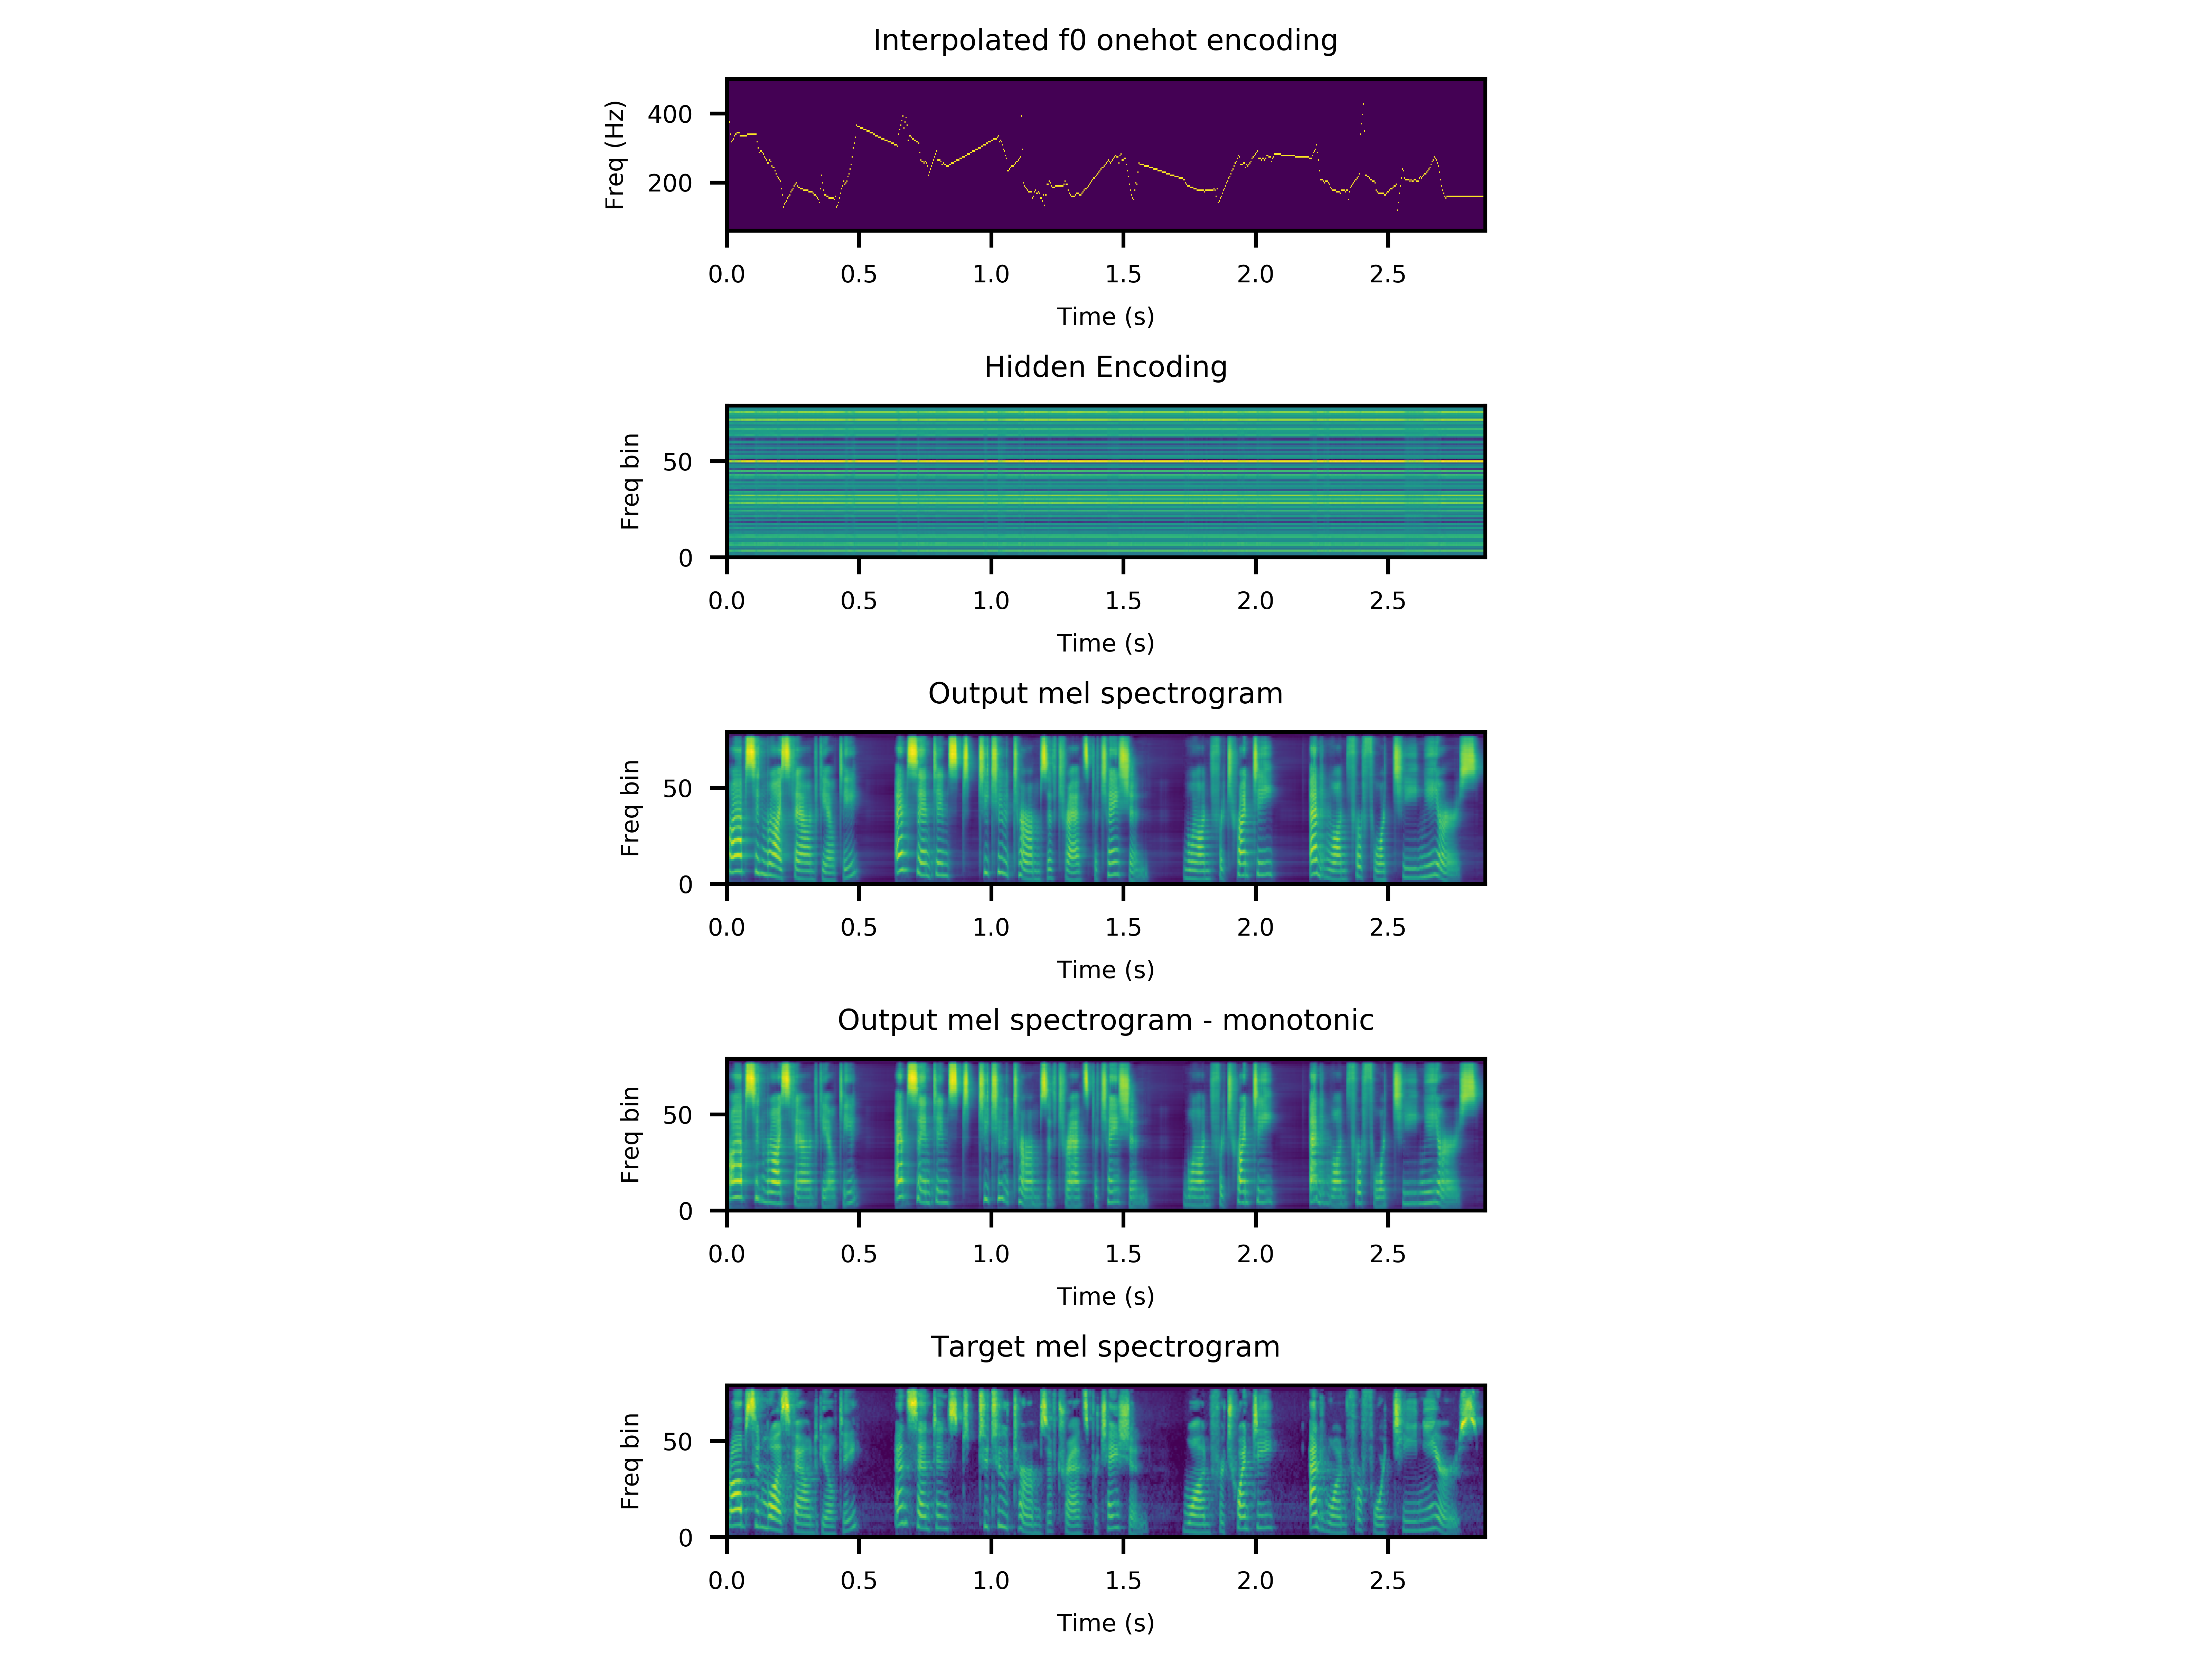
\includegraphics[width=\textwidth,trim={3.8cm 0cm 4.8cm 5cm},clip]{figures/beta-100-spects_step-12750-0y0939.png}
    \caption{$\beta$ = 200}
    \label{fig:1beetbig}
  \end{subfigure}
  %
  \begin{subfigure}[b]{0.45\textwidth}
    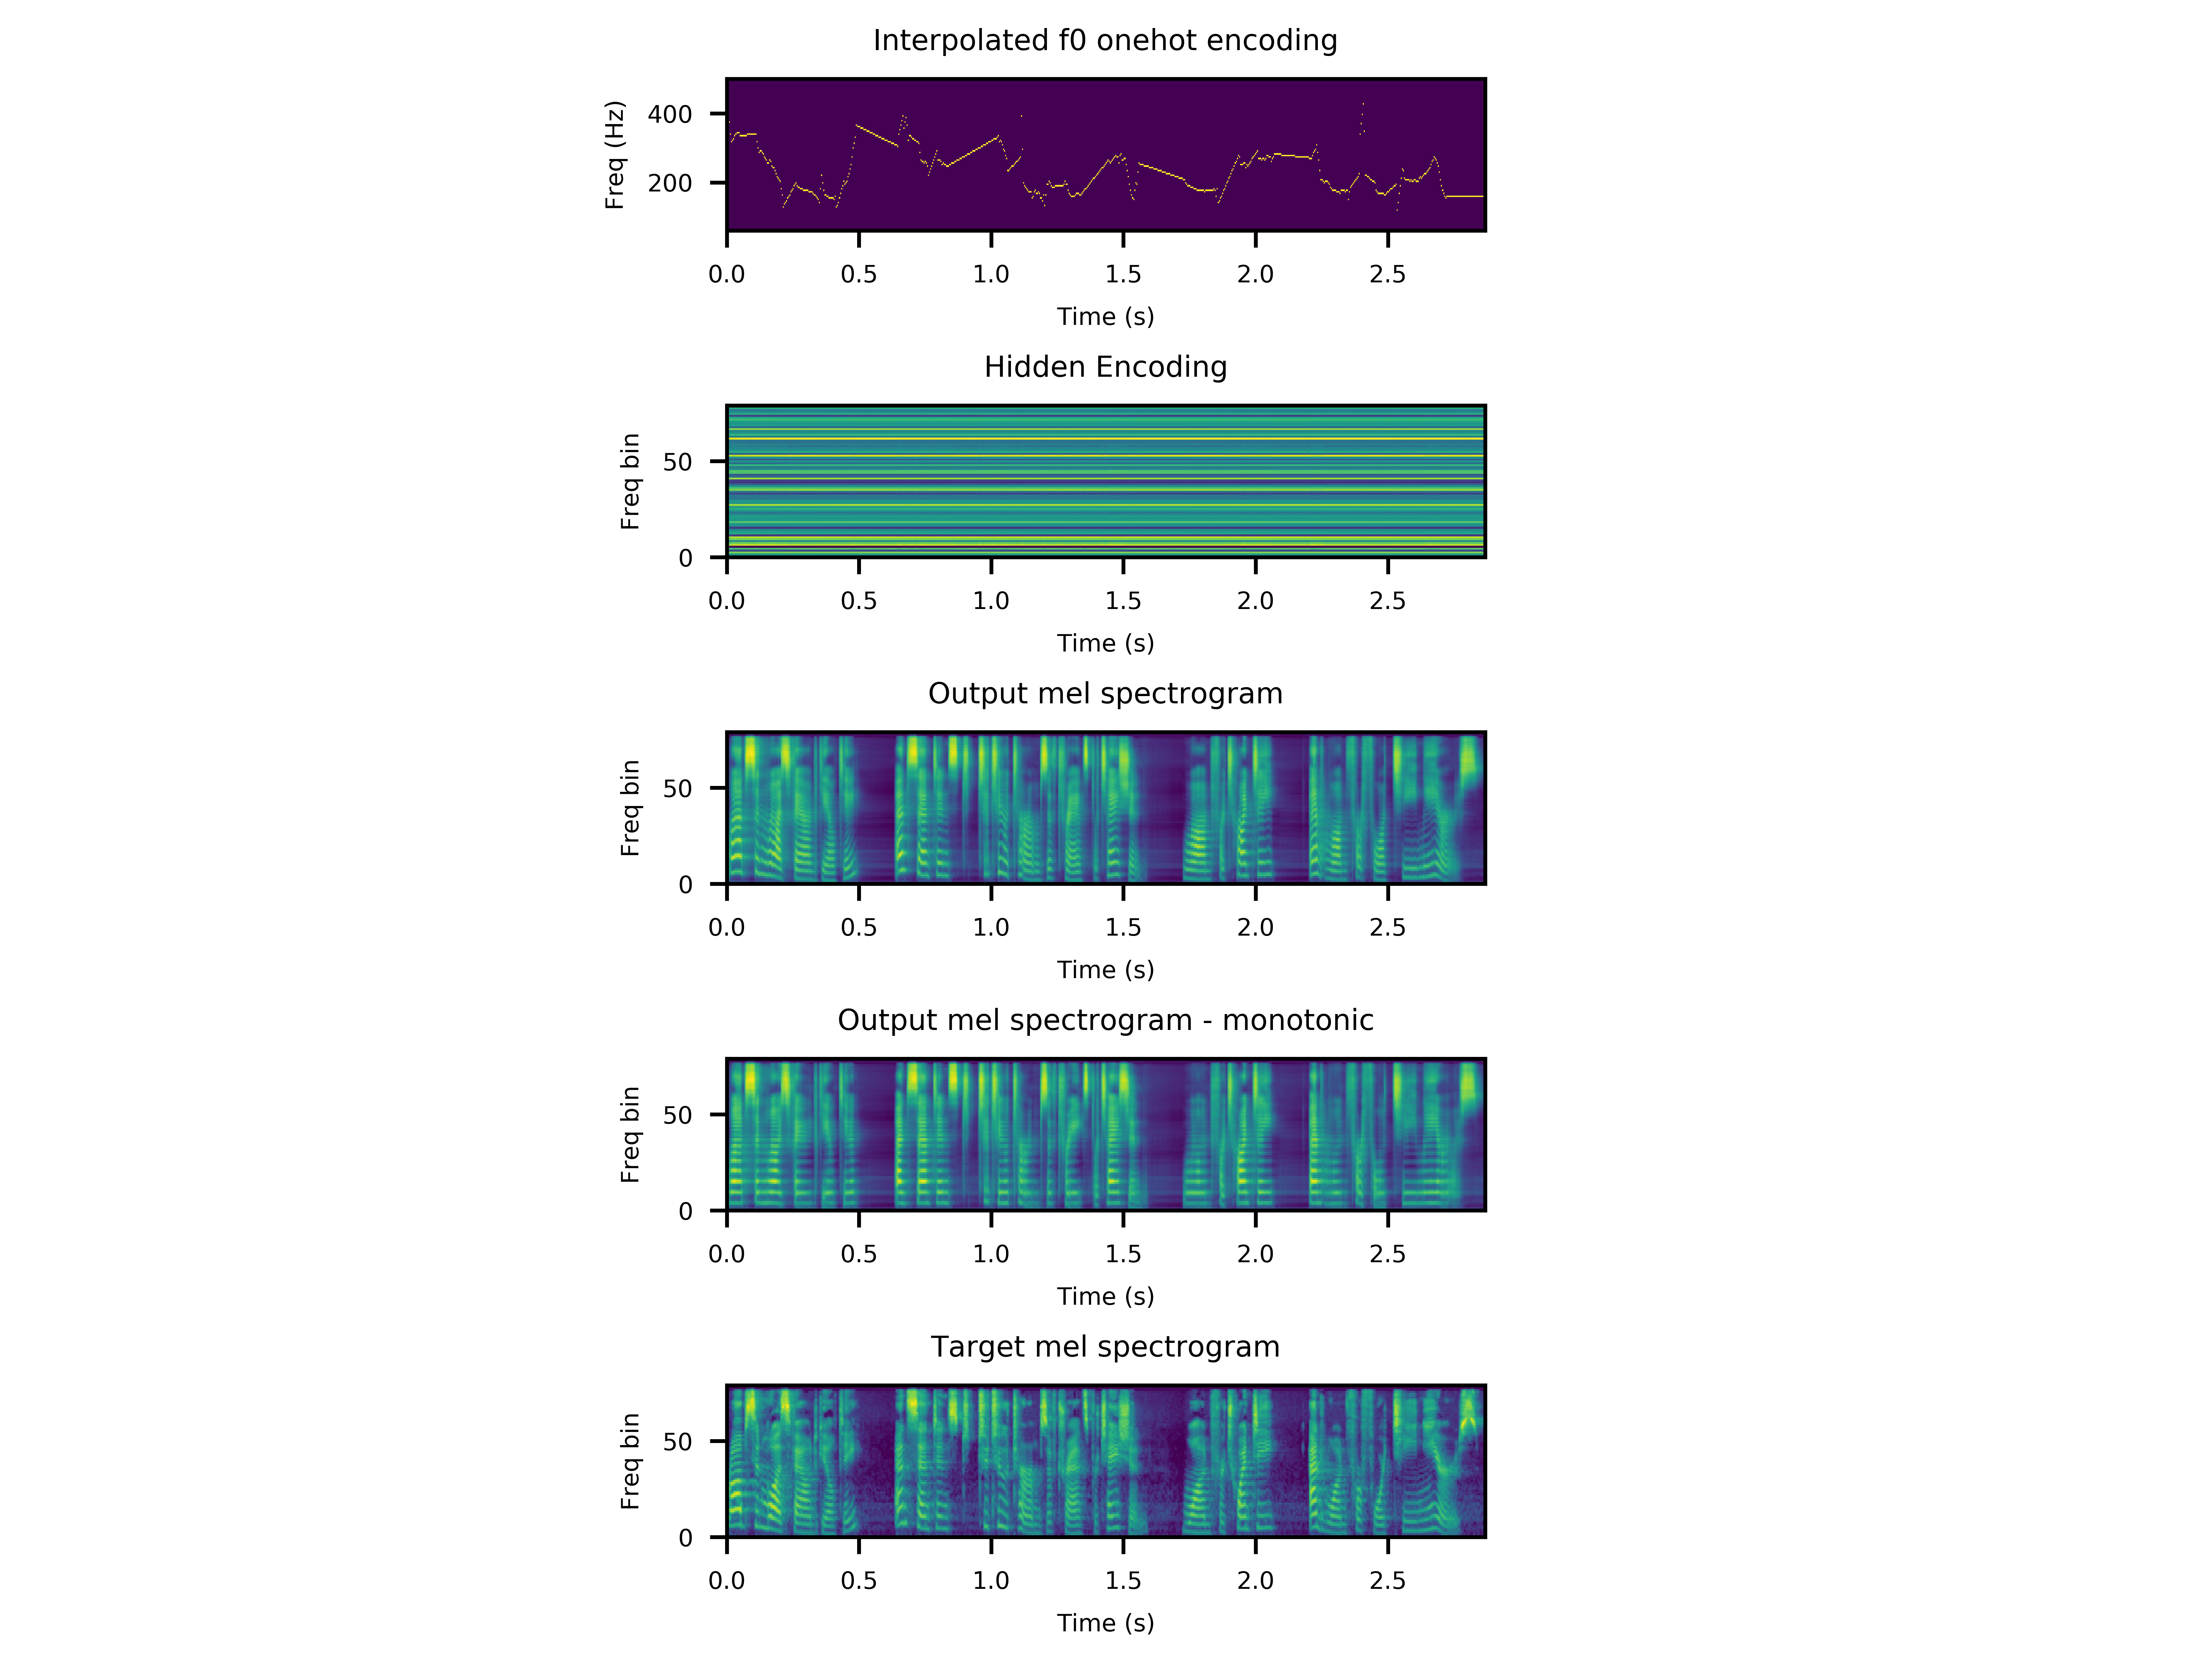
\includegraphics[width=\textwidth,trim={3.8cm 0cm 4.8cm 5cm},clip]{figures/beta-800-spects_step-12900-0y1095.png}
    \caption{$\beta$ = 800}
    \label{fig:2big}
  \end{subfigure}
\end{figure}

\end{frame}


\begin{frame}{Lessons}
The hypothesis is sound: reducing information in $h$ means system does not ignore $y$

Quality is degraded along the way:

audio $\to$ spectrum $\to$ modified-spectrum $\to$ modified-audio

Have only tested with one parameter that it is fairly easy to modify using DSP
\end{frame} 

\section{Future Work}

\begin{frame}{Overview}
    \begin{enumerate}
        \item Improve quality (next 3 months)
        \item Add loss function for fidelity to $y$ in output
        \item Try other parameters other than F0 -- spectral slope etc.
        \item Try parameters that are \emph{global} as well as \emph{local}
        \item Investigate seq2seq models for this -- hide higher level features e.g. language
        \item Use control parameters of physical significance, where training data is output of physical models
    \end{enumerate}
\end{frame}


\begin{frame}{Improving Quality}
A task for the next few months... a few approaches
\begin{enumerate}
    \item explore more hyperparameters/architectures for component networks
    \item try out different vocoders 
    \begin{itemize}
        \item currently only use pretrained Amazon Universal
        \item introduces artefacts
        \item develop own vocoder?
    \end{itemize}
    \item train vocoder on artificial output
\end{enumerate}

\end{frame}
\subsection{Next 3 Months}

\appendix
\begin{frame}[fragile]{Leakage Loss}
\begin{equation}
\label{eq:ladver}
    \mathcal{L}_{adversarial} = \alpha \cdot \mathcal{L}_{combiner} + \beta \cdot \mathcal{L}_{leakage}
\end{equation}


\begin{equation}
\label{equation:leak}
    \mathcal{L}_{leakage} = \textup{Var}(\textup{softmax}(\textup{finder}(\textup{hider}(x))))
\end{equation}

Where $Y$ is dist of $y$ across all categories

\begin{equation}
    Y | x = \textup{softmax}(\textup{finder}(\textup{hider}(x))).
\end{equation}

\begin{equation}
\label{equation:leak2}
    \mathcal{L}_{leakage} = \textup{Var}(Y | x).
\end{equation}

\end{frame}

\end{document}
